Based on the requirements and specifications presented in the previous chapters, the architecture was designed as shown in the following figure \ref{architecure}:
\begin{figure}[H]
	\centering
	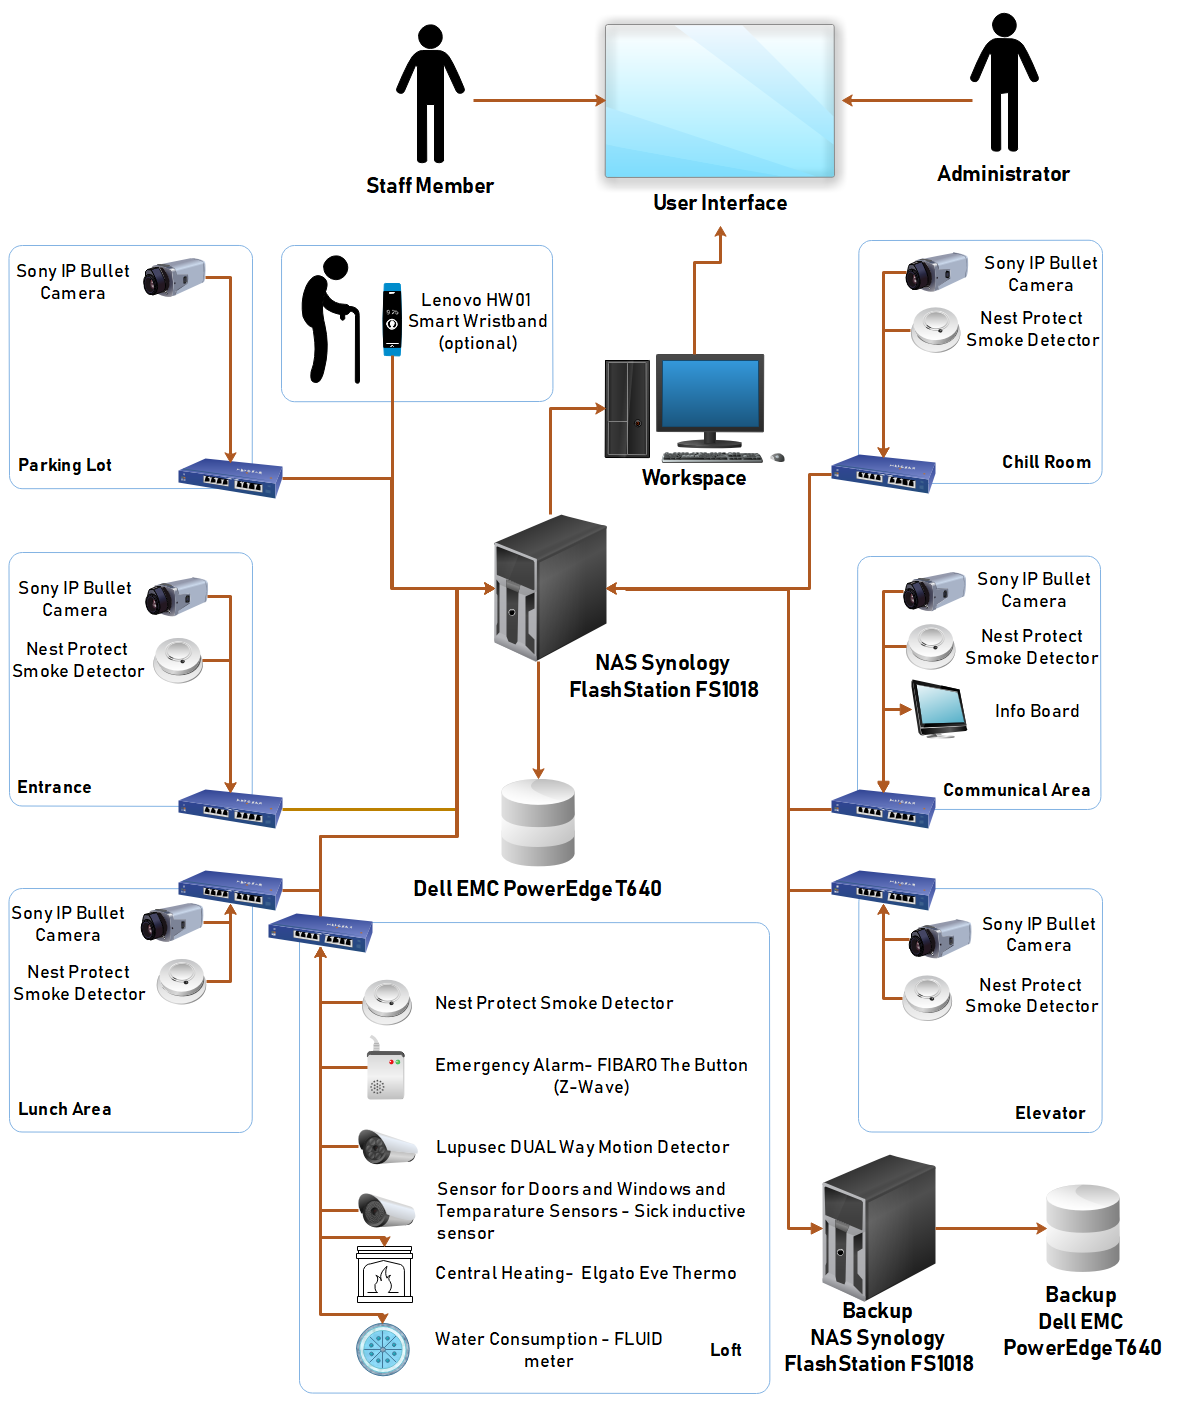
\includegraphics[width =1.0\textwidth]{.images/architecture.PNG}
	\caption{Basic architecture}
	\label{architecure}
\end{figure}
The figure shows the central hardware components of the iCare system and the connected devices. The rectangles represent the different rooms of the building. Each room has a HUB that communicates with the central server of the iCare system. In each room, the devices shown in the associated rectangle are installed as part of the iCare system, which communicate with the room's HUB via a wireless connection. This way, the required data reaches the server and is persisted in a database if required. The iCare server uses a RAID 2 backup system with a backup database to ensure the safety of the aquired data. The data can be accessed by employees or the administrator from any workspace using a web user-interface. The authorisation specified in the specification applies to the access to areas which show protected contents. In addition, patients can be given wristbands which monitor their vital functions on a voluntary basis or by order of a doctor. These wristbands communicate with the central server via a wireless connection and transmit the recorded data in real time.